\chapter{Generic interface}\label{app:generic-interface}

Generic interface is an internal name for a certain custom functionality. It is not a common term. However it is derived from generic types. Something that is often used in typed programming languages.

\section{The flow of the generic interface}
    \begin{enumerate}
        \setlength\itemsep{-2pt} 
        \item{A user sends a request that contains a certain query. The query can be seen as a predefined structure comparable to an SQL query, but with more capabilities to filter and on a higher level.}
        \item{Although I am not completely aware of the inner working, the generic interface maintains / collects data from different sources based on the provided query.}
        \item{The gathered data is filtered based on that same query.}
        \item{A response is sent back to the user in the shape of a flattened table.}
    \end{enumerate}  
     \begin{figure}[H]
        \centering
        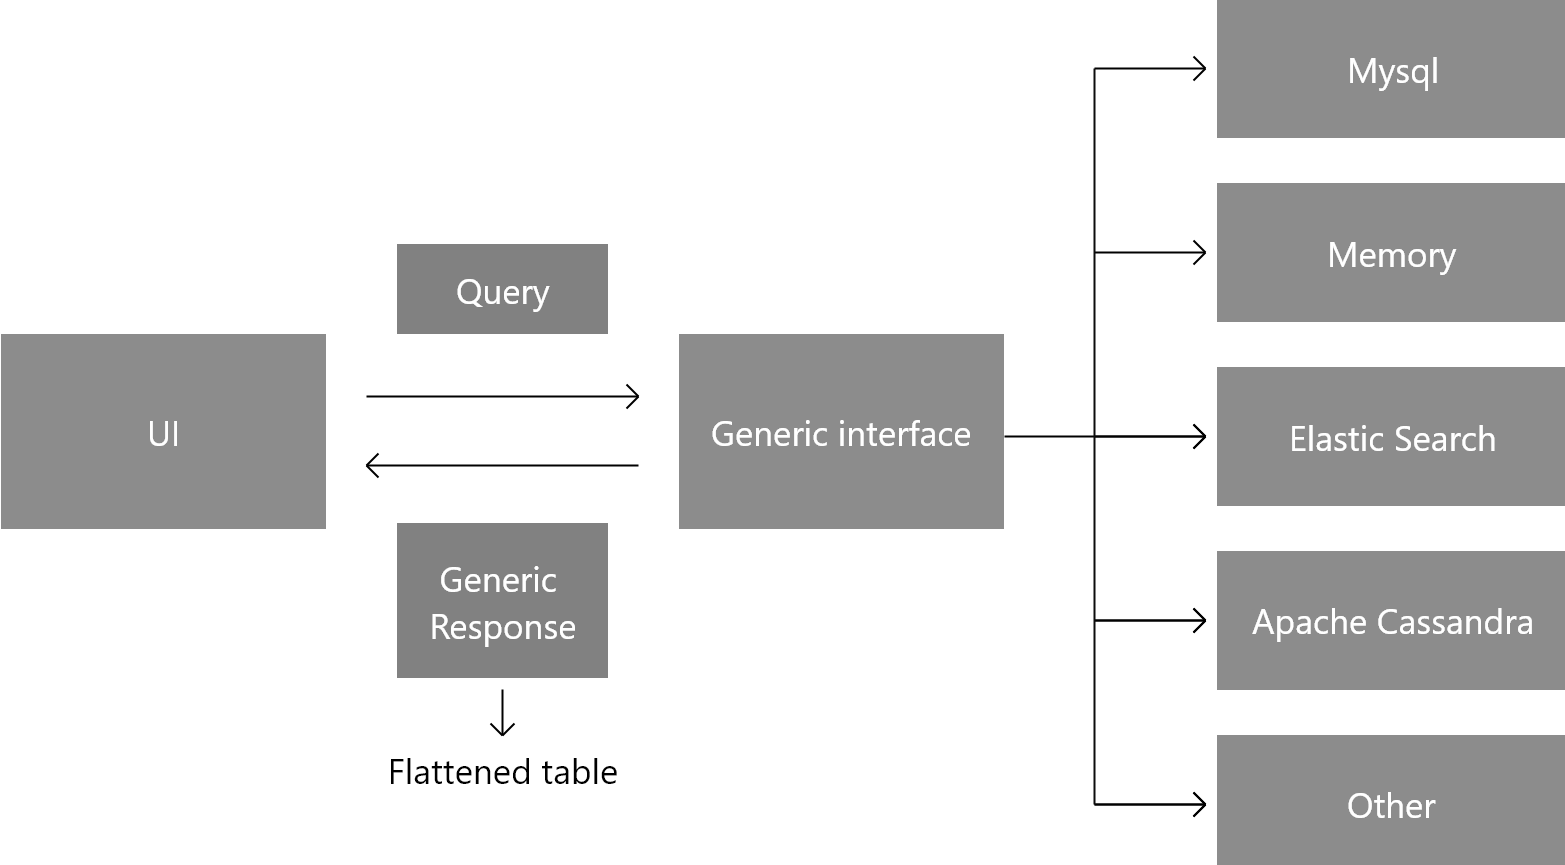
\includegraphics[scale=0.20]{generic-interface-flow.png}
        \caption{diagram generic interface}
        \label{fig:diagram-generic-interface}
    \end{figure}
    
\section{Flattened table}

\subsection{Denormalized table}
Imagine you have product data that you want to store in a database. In case you store the data like \autoref{tab:denormalized}, it is stored as a flat table. All the information is stored in a single table.

\begin{table}[H]
\begin{tabular}{ | l | l | l | l |}
    \toprule
    \textbf{Id}     & \textbf{Product name} & \textbf{material}     & \textbf{category}  \\
    \midrule
    1               & Computer keyboard     & Plastic                   & computer peripherals     \\
    \midrule
    2               & Computer mouse        & plastic                   & computer peripherals      \\
    \midrule
    3               & Adobe XD              & n.a.                      & computer software         \\
    \midrule
    4               & Monitor               & Aluminium                 & computer peripherals      \\
    \bottomrule
\end{tabular}
\centering
\captionsetup{justification=centering}
\caption{Denormalized table}
\label{tab:denormalized}
\end{table}

\subsection{Normalized tables}
Normalization is a technique where you decompose tables to eliminate data redundancy. In this example the denormalized table is normalized into 2 separate tables. \autoref{tab:normalized-product}, which is the product table. \autoref{tab:normalized-category}, which is the category table.

Notice that the value \textit{computer peripherals} is stored only once instead of 3 times. This is a major advantage. Not because we avoid data duplication but because we enforce data integrity. Because of the relation between the product table and the category table, it is no longer possible to delete the category \textit{computer peripherals}, or any other category that is in use. It may seem like the flat structure is a bad structure. A flat structure is great for reporting and analytics.

Flattening refers to the process of denormalizing a normalized database. From \autoref{tab:normalized-category} and \autoref{tab:normalized-category} to \autoref{tab:denormalized}.

In case of the generic interface, data from different sources is joined together in one large flattened table without any relations.

\begin{table}[H]
\begin{tabular}{ | l | l | l | l |}
    \toprule
    \textbf{Id}     & \textbf{Product name} & \textbf{material}     & \textbf{category}  \\
    \midrule
    1               & Computer keyboard     & Plastic                   & 1     \\
    \midrule
    2               & Computer mouse        & plastic                   & 1     \\
    \midrule
    3               & Adobe XD              & n.a.                      & 2     \\
    \midrule
    4               & Monitor               & Aluminium                 & 1     \\
    \bottomrule
\end{tabular}
\centering
\captionsetup{justification=centering}
\caption{Normalized product table}
\label{tab:normalized-product}
\end{table}

\begin{table}[H]
\begin{tabular}{ | l | l |}
    \toprule
    \textbf{Id}     & \textbf{Category name}\\
    \midrule
    1               & computer peripherals  \\
    \midrule
    2               & Computer software     \\
    \midrule
    \bottomrule
\end{tabular}
\centering
\captionsetup{justification=centering}
\caption{Normalize category table}
\label{tab:normalized-category}
\end{table}
